% News & generic usage

Modern media and news distribution is shifting from traditional media to social media.
Modern media production and information distribution is shifting from traditional outlets.
Also media consumption is shifting from traditional outlets to digital and mobile devices.
from con-sumer to pro-sumer.
Niet gebonden aan expert opinion / editorial, maar aan eigen mening zonder professionele studio / news desk / kantoor; maar juist mobile eye-witness; direct van individu naar massa!

% Social journalism
Social media has been a driving force in the Arab Spring 
Multi-media 
Camera phones
People have used social media to reach 20 million 


excludes large portions of the global dialog on social media.


%What advantages does a smart phone have compared to a laptop and desktop?
Given this context mobile devices are increasingly important and smart-phone in particular.
A smart-phone has the unique property of being a ubiquitous device that is highly mobile and extremely connectible.
Most smart-phones even have one or more cameras to produce multi-media content that can be shared immediately from the device.
Finally the entire world has a smart-phone.
Even or especially areas without tradition infrastructure they are ubiquitous.

% Communication in crisis situations

In crisis situations, like natural disaster or unrest, the smart-phone becomes particularly important, exactly for the earlier mentioned properties, as under such conditions utilizing centralized infrastructure is undesired (censorship) or physically impossible.
Decentralized can work in these situations.
Censorsihp and large scale monitoring is difficult in decentralized networks.
Refereren aan article Johan 2011 voorbeeld.

Internet is in danger....

%Unavailable infrastructure

Internet kill-switches

Overloaded

Physically destroyed

%first point
With servers central to their design they create a single point of failure, even in a decentralized set-up.
Several natural disasters have taken out the necessary infrastructure on numerous occasions for a prolonged period of time.
%examples
Especially in situations like these, people need to communicate and coordinate their efforts to restore safety.
Social media has played a major role in recent calamities when people could mark themselves as safe, effectively broadcasting that information to all their family and friends on social media, instead of contacting them one by one or not at all due to congestion in the communication channels.
So the advantages are obvious, and the vulnerability of central elements underlying current social media too.


%Untrusted infrastructure

Censorship

Partly disconnected

%second point
The lack of anonymity becomes a problem when the users privacy is being invaded.
Revealing personal information can be deduced from search queries for example, or associations on social platforms.
When this information can be used for targeted advertising it becomes very valuable, and creates an incentive for the parties that have access to this information to sell it to third parties.
In fact the business model of social media appears to be serving targeted advertisements to its users on behalf of third parties.
What's even worse is social media integrated into regular websites to de-anonymize and track the whereabouts of users even outside of the social media realm.
Whenever users lose control over their privacy it becomes a serious problem.




% Internet censorship
The Internet makes it easy to communicate freely on a global scale.
Connecting to it and crossing international borders on-line does not require approval of any governmental body.
This freedom due to the absence of oversight and control allows anyone with the capability to monitor, filter, delay, or block Internet traffic at will.
Internet exchange (IX) infrastructures are among the central components in the inter-network architecture that are particularly vulnerable to large scale abuse, even beyond total monitoring and filtering.
As such, not everyone has unrestricted access to the Internet due to censorship and surveillance.
In fact a significant part of today's Internet users is affected by these attempts to hide or distort reality. %ref
This interference directly affects the universal right to freedom of opinion and expression as stated in article 19 of the Universal Declaration of Human Rights (UDHR).

% Privacy
Pervasive monitoring of digital citizens by Internet providers on behalf of governments to enforce censorship laws raises severe privacy concerns.
Even the business model of social media companies directly conflicts with user privacy.
Targeted advertising requires the very information of high quality (accurate and current) users tend to share with their friends on-line.
When this information is shared with other parties outside of the specific social media website, possibly unknowingly to the user, it effectively becomes a privacy leak.
Subsequently users can be confronted with their information being misused in various ways beyond their control.
This lack of control over your own privacy can lead to arbitrary interference as defined in UDHR article 12. %ref, example, human rights watch, nelie kroes, etc.
Integration of social media on regular websites aggravates this problem.
Every page-view and click on social media enabled websites becomes traceable to an individual, directly benefiting the business model of targeted advertisements

% Internet censorship 2
The incentive to de-anonymize the user, not only causes a lack of privacy, but also a potential lack of freedom of expression, as it hands key information to the censor: who is expressing dissent and who is associated with this person on-line.
Cyber suppression has become a reality when you no longer can be associated with opinion-makers or foreign journalists on-line.




The sophistication of censorship techniques is pushed forward by the drive to stay ahead of attempts trying to circumvent it.
Increasingly though, Internet traffic is put under surveillance and obfuscation techniques are targeted by restrictions.


fragmentation of efforts for freedom


\section{Adversary model}
\pagebreak

\begin{figure}[h]
	\centering
	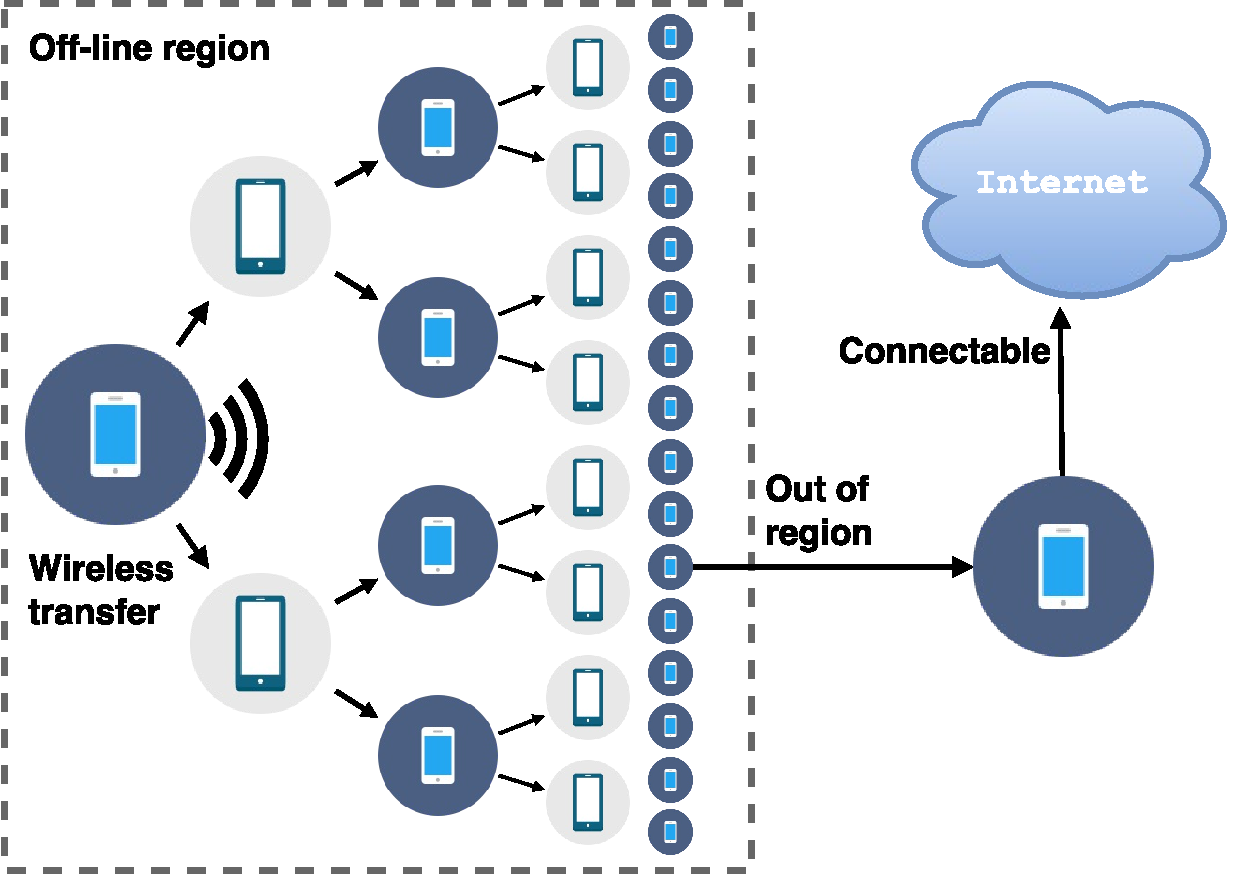
\includegraphics[width=\textwidth]{viral_spreading}
	\caption{Any device can spread to other devices wirelessly.
		Only one device has to travel or connect outside the offline region to make the content connectable to the Internet.}
	\label{fig:viral_spreading}
\end{figure}



%scope
To ensure that no controlling party can exercise censorship we distribute authority over all users, creating an \emph{autonomous} system.
If all information is located in one or a few places, the parties in charge of that location will still have control over it, so we must distribute information over all users, creating a \emph{communication} system.
Then if all users want to use this system to share, order and appreciate each others information, in other words the essence of social media: social interaction, with everyone being able to interact in the same way, we need to  distribute functionality over all users, creating a \emph{cooperation} system.
Fully distributed systems capture these characteristics. %move to solution?
Without any central component in the system it is no longer susceptible to censorship without everyone participating.

Peer-to-peer communication technology is essential for a server-less distributed system.
Mobile devices typically do not require infrastructure to exchange information, like those equipped with Bluetooth or capable of ad hoc Wi-Fi.
Smart phones are ubiquitous everywhere in the world and used to access social media and retrieve information from the Internet.
Fortuitously these are also the type of mobile devices that can communicate peer-to-peer.






\section{Explore environment}
% learn about domain
% current state of technology
% what others before me have researched and accomplished

Various initiatives have been started to deal with one or both of these problems.
Figure \ref{fig:youbroketheinternet} shows a mapping of projects that are or have been working on that.
%From re-decentralized: top projects that match/compare.
\\
\begin{figure}[h]
	\centering
	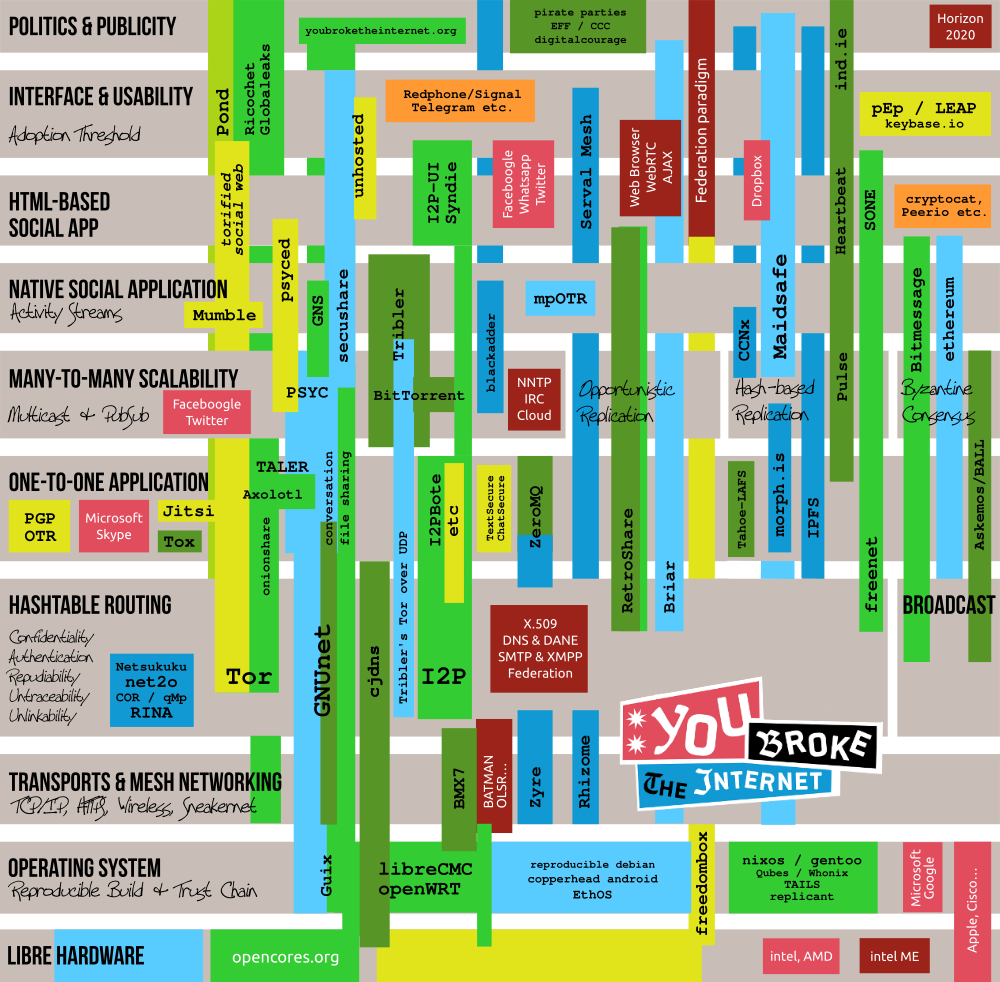
\includegraphics[width=\textwidth]{youbroketheinternet}
	\caption{Map of projects trying to fix the Internet according to youbroketheinternet.org, last updated October 2015\\
		\\
		Colour coding:\\
		\\
		\textcolor[RGB]{51,204,51}{Green:} Projects that are available today.\\
		\textcolor[RGB]{86,149,38}{Dark green:} Projects that are available, but are not fully protective of meta-data.\\
		\textcolor[RGB]{89,204,255}{Blue:} Projects in development.\\
		\textcolor[RGB]{17,153,211}{Dark blue:} Projects in development which will have little or no protection of meta-data (but that does not mean they can't be an excellent piece in the general puzzle).\\
		\textcolor[RGB]{226,228,27}{Yellow:} Projects that may be okay but depend too much on the security of servers.\\
		\textcolor[RGB]{255,153,51}{Orange:} Products whose end-to-end encrypting client side has been open-sourced but whose server side remains proprietary.\\
		\textcolor[RGB]{225,77,93}{Red:} Brands that currently occupy the respective layers with unsafe technology.\\
		\textcolor[RGB]{155,35,25}{Dark red:} Possibly cool but unsafe technologies that we need to replace.}
	\label{fig:youbroketheinternet}
\end{figure}


